%------------------------------------ Inicio ---------------------------------------
\documentclass[11pt, a4paper]{article}

% -------------- Nombre del documento --------------
\newcommand{\nombre}{TP 4}
%---------------------------------------------------------

%-------------------- Include Paquetes iniciales---------------------
\usepackage{mathtools}
\usepackage{graphicx}
\usepackage{float} 
\usepackage{geometry}
\geometry{top=35mm,bottom=30mm,left=33mm,right=33mm,headsep=15mm}
\usepackage{relsize} % agranda a un mas las letras
\usepackage[spanish,es-nodecimaldot]{babel}
\usepackage[utf8]{inputenc}
\usepackage{lastpage} % nos dice el numero total de paginas
\usepackage{fancyhdr} % modifica encabezado y pie de pagina
\pagestyle{fancy} % Con ésto aplicamos el encabezado y pie 
\renewcommand{\headrulewidth}{0.2pt} % linea encabezado tamaño
\renewcommand{\footrulewidth}{0pt} % linea pie de pagina tamaño

\cfoot{}
\pagestyle{fancy}
\fancyhf{}
\rfoot{\thepage}
\lhead{
\includegraphics[scale=0.12]{Imagenes/logounc.jpg}}
\rhead{\nombre}
%-----------------------------------------------------------------------


\begin{document}

%--------------------  Portada ---------------------


\begin{center}
	{\huge\textbf{SINTESIS DE REDES}} \\
	\vspace{3mm}
	{\huge\textbf{ACTIVAS}} \\
	\vspace{10mm}
	{\large -}
	\vspace{2mm}
	
\begin{figure}[H]
	\centering
	
\includegraphics[width=0.7\linewidth]{Imagenes/logoPrincipal.png}
\end{figure}
\vspace{10mm}
\textscale{3}{ \textbf{\nombre}} \\
\vspace{8mm}
\textscale{1.6}{ Filtros activos\textbf{}}\\
\vspace{6mm}
	\textscale{1.3}{ Síntesis de Redes Activas - 2024\textbf{}}\\
	\vspace{15mm}
	---------------------------------------------\-\\
	\vspace{15mm}
	\textscale{1.3}{\textbf{Integrantes}}\\
	\vspace{6mm}
	\textscale{1.3}{Valentin Jose Ramirez, 43700362}\\
 \vspace{2mm}
	\textscale{1.3}{José Ignacio Lopez Sivilat, 44805902}\\
 \vspace{2mm}
	\textscale{1.3}{Franco Gabriel Lopez, 43271762} \\
     \vspace{2mm}
	\textscale{1.3}{Alejo Adrian Beierbach, 43700333} \\
	\vspace{15mm}
	\textscale{1.3}{\textbf{Profesores adjuntos}}\\
 \vspace{6mm}
 \textscale{1.3}{Dr. Ing. Pablo A. Ferreyra}\\
 \vspace{2mm}
 \textscale{1.3}{Ing. César Reale}\\
	\thispagestyle{empty}
\end{center}
\clearpage
%----------------------------fin portada-----------
\thispagestyle{empty}
\tableofcontents
\clearpage


% ------------------------------------- Desarrollo ---------------------------------
\pagenumbering{arabic}


\section{Introducción a los Osciladores}

Un oscilador es un dispositivo capaz de generar señales periódicas, comúnmente en forma de ondas sinusoidales, cuadradas o triangulares, sin la necesidad de una entrada continua externa. Los osciladores se utilizan ampliamente en diversas aplicaciones, tales como sistemas de comunicación, relojes electrónicos, y circuitos digitales. 

En general, los osciladores pueden clasificarse en:
\begin{itemize}
    \item \textbf{Osciladores sinusoidales:} Generan señales continuas suaves, como los osciladores LC o RC.
    \item \textbf{Osciladores no sinusoidales:} Producen señales con transiciones abruptas, como los osciladores de anillo o los multivibradores.
\end{itemize}

El diseño y análisis de un oscilador se centra en garantizar la estabilidad y precisión de la señal generada, lo cual depende de los componentes utilizados y del entorno de operación.

\section{Osciladores de Anillo}

El oscilador de anillo es un tipo de oscilador no lineal que consiste en un número impar de etapas inversoras conectadas en forma de anillo cerrado. Este tipo de oscilador es ampliamente utilizado en circuitos digitales debido a su simplicidad y facilidad de implementación.

\subsection{Principio de Funcionamiento}

El oscilador de anillo funciona gracias a la retroalimentación negativa y al retardo de propagación inherente de cada etapa. La señal recircula a través de las compuertas inversoras, generando oscilaciones periódicas. Para que el circuito oscile, es necesario que:
\begin{itemize}
    \item El número de etapas inversoras sea impar, para garantizar la inversión lógica.
    \item El retardo total del circuito permita cumplir las condiciones de oscilación.
\end{itemize}

La frecuencia de oscilación está determinada por el tiempo de propagación de las etapas y se puede expresar como:
\[
f = \frac{1}{2n \cdot t_p}
\]
donde \(n\) es el número de etapas y \(t_p\) es el tiempo de propagación de cada inversor.

\subsection{Configuración Básica}

Un oscilador de anillo típico utiliza inversores CMOS conectados en serie, con el último inversor retroalimentado a la entrada del primero. Este diseño aprovecha las capacidades parasitarias de los inversores para mantener las oscilaciones.


   \begin{figure}[H]
    \centering
    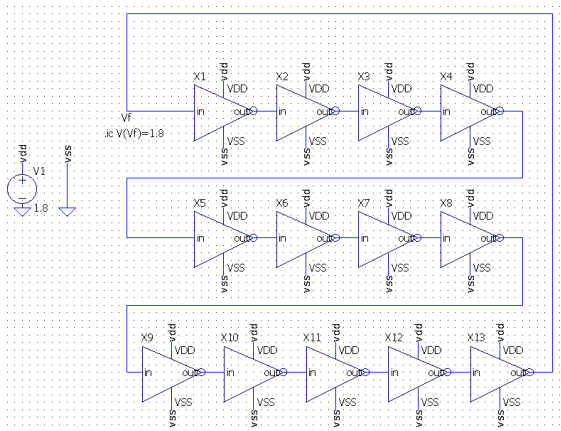
\includegraphics[width=0.8\textwidth]{Imagenes/Oscilador1.png}
    \caption{Oscilador de anillo}
    \label{fig:Oscilador1}
    \end{figure}
 
\section{Componentes y Configuración}

\subsection{Diseño del Oscilador de Anillo}

Para este trabajo práctico, se diseñará un oscilador de anillo utilizando 13 inversores conectados en serie. El diseño y simulación se realizarán en el software LTspice, considerando las siguientes especificaciones:

\begin{itemize}
    \item Número de etapas: \( n = 13 \) (impar para garantizar la oscilación).
    \item Tensión de alimentación: \( V_{DD} = 1 \, \mathrm{V} \).
    \item Tiempo de propagación por inversor: \( t_p = 10 \, \mathrm{ns} \).
    \item Nivel de disparo (\( V_M \)): \( V_M = 0.5 \cdot V_{DD} = 0.5 \, \mathrm{V} \).
    \item Capacidad de carga por inversor: \( C_L = 10 \, \mathrm{pF} \).
    \item Criterio del 50\%: Se tomará como referencia el cruce por el nivel \( V_M \) para calcular el retardo y evaluar la oscilación.
\end{itemize}

\subsection{Cálculo de la Frecuencia de Oscilación}

La frecuencia de oscilación (\( f \)) de un oscilador de anillo se determina a partir del tiempo de propagación (\( t_p \)) de cada etapa y el número total de etapas (\( n \)):

\[
f = \frac{1}{2n \cdot t_p}
\]

Sustituyendo los valores especificados:
\[
f = \frac{1}{2 \cdot 13 \cdot 10 \, \mathrm{ns}} = \frac{1}{260 \, \mathrm{ns}} \approx 3.85 \, \mathrm{MHz}
\]

\subsection{Simulación en LTspice}

El circuito será implementado en LTspice siguiendo estos pasos:
\begin{enumerate}
    \item Diseñar un inversor CMOS utilizando transistores MOSFET ideales con características compatibles con \( V_{DD} = 1 \, \mathrm{V} \).
    \item Conectar 13 inversores en serie, formando un bucle cerrado.
    \item Agregar una carga capacitiva \( C_L = 10 \, \mathrm{pF} \) a la salida de cada inversor.
    \item Configurar la simulación para medir el voltaje de salida de una etapa y determinar su comportamiento periódico.
    \item Establecer el punto de medición del retardo considerando el cruce por \( V_M = 0.5 \, \mathrm{V} \).
\end{enumerate}

\subsection{Resultados Esperados}

Se espera que la señal de salida del oscilador sea una onda cuadrada con una frecuencia cercana a los \( 3.85 \, \mathrm{MHz} \). Los resultados obtenidos a partir de la simulación en LTspice serán comparados con el valor teórico calculado para validar el diseño.

\section{Simulación de un Inversor CMOS}

Antes de diseñar el oscilador de anillo completo, se realizará una simulación preliminar de un único inversor CMOS en LTspice. Esto permitirá caracterizar su comportamiento dinámico y validar el tiempo de propagación (\( t_p \)) bajo las condiciones especificadas.

\subsection{Diseño del Inversor CMOS}

El inversor CMOS estará compuesto por:
\begin{itemize}
    \item Un transistor MOSFET tipo \( p \) (PMOS) conectado a \( V_{DD} = 1 \, \mathrm{V} \).
    \item Un transistor MOSFET tipo \( n \) (NMOS) conectado a tierra (\( GND \)).
    \item La entrada común a las puertas de ambos transistores.
    \item La salida común a los drenadores de los transistores, con una capacidad de carga \( C_L = 10 \, \mathrm{pF} \).
\end{itemize}

El punto de disparo del inversor estará centrado en \( V_M = 0.5 \cdot V_{DD} = 0.5 \, \mathrm{V} \), y se tomará como referencia para evaluar el retardo.

El circuito de un inversor CMOS es el siguiente:



   \begin{figure}[H]
    \centering
    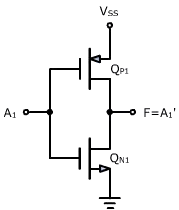
\includegraphics[width=0.4\textwidth]{Imagenes/inversorcmos.png}
    \caption{Inversor CMOS}
    \label{fig:inversorcmos}
    \end{figure}




El principio de funcionamiento es el siguiente, cuando la señal de entrada es un "0", esta en 0V la entrada y por lo tanto también los gate de los transistores están en 0V, por lo tanto, el MOSFET de canal n tiene una Vgs de 0 V ya que su source esta a 0V, por lo que este transistor se corta y no deja pasar la corriente (se pone en un estado de alta impedancia), en cambio, en MOSFET de canal P tiene una Vgs igual a VDD por lo que este se prende (se pone en un estado de baja impedancia), bajo estas condiciones nos quedaría un circuito similar al de un divisor resistivo, pero la resistencia conectada a VDD es de un valor muy bajo, y la resistencia conectada a GND es de un valor extremadamente alto, entonces a la salida se ve un valor de tensión cercano a VDD ("1").

Cuando la entrada es un "1", los gate de los transistores están a VDD, se produce el efecto contrario al comentado anteriormente, quedando la resistencia que esta conectada a VDD de un valor extremadamente alto y la resistencia conectada a GND en un valor muy bajo, por lo que a la salida se ve un valor de tensión cercano a 0V ("0")

\subsection{Simulación en LTspice}

Para caracterizar el inversor, se seguirán estos pasos:
\begin{enumerate}
    \item Implementar el circuito del inversor CMOS en LTspice utilizando transistores MOSFET ideales o modelos compatibles con \( V_{DD} = 1 \, \mathrm{V} \).
    \item Configurar una entrada pulsada (\texttt{PULSE}) con:
    \begin{itemize}
        \item Niveles: \( 0 \, \mathrm{V} \) a \( V_{DD} \).
        \item Tiempo de subida y bajada: \( 1 \, \mathrm{ns} \).
        \item Frecuencia: suficiente para observar la respuesta transitoria.
    \end{itemize}
    \item Agregar una capacidad de carga \( C_L = 10 \, \mathrm{pF} \) en la salida.
    \item Realizar una simulación transitoria para medir:
    \begin{itemize}
        \item El tiempo de propagación (\( t_p \)) midiendo los tiempos de cruce al nivel \( V_M = 0.9 \, \mathrm{V} \) en la entrada y salida.
        \item La forma de onda de salida para verificar el comportamiento esperado.
    \end{itemize}
\end{enumerate}

\subsection{Resultados Esperados}

Se espera que la salida del inversor CMOS sea una forma de onda inversa con respecto a la entrada, mostrando un retardo característico. El tiempo de propagación (\( t_p \)) se medirá como el promedio entre:
\[
t_p = \frac{t_{PLH} + t_{PHL}}{2}
\]
donde \( t_{PLH} \) es el tiempo de propagación de bajo a alto, y \( t_{PHL} \) de alto a bajo. Este valor deberá estar próximo a \( 10 \, \mathrm{ns} \), como especificado.

\subsection{Resultados Obtenidos}
El esquemático utilizado fue el siguiente:
   \begin{figure}[H]
    \centering
    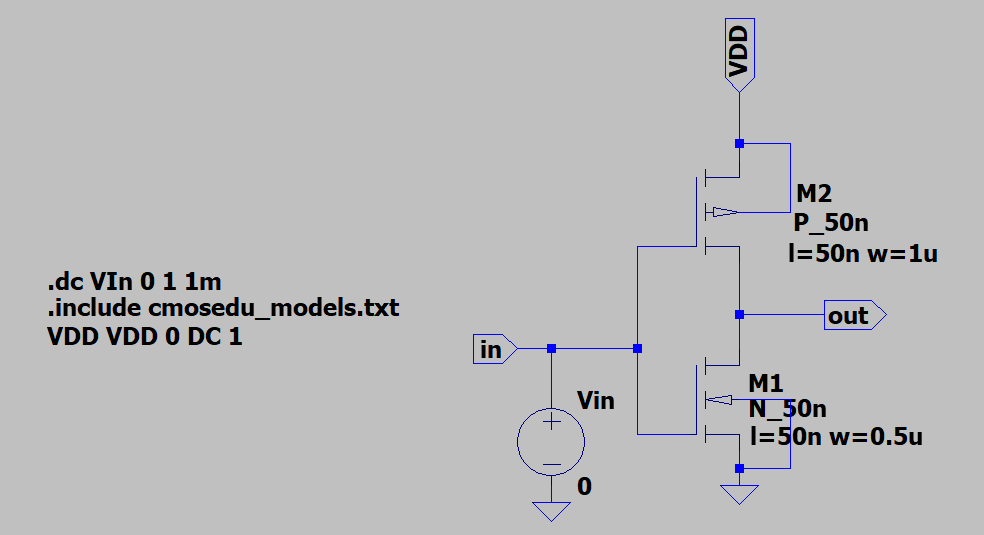
\includegraphics[width=0.8\textwidth]{Imagenes/esquematico.png}
    \caption{Esquemático utilizado}
    \label{fig:esquematico}
    \end{figure}

 Se utilizaron transistores de la librería N\_50n y P\_50n, los cuales tienen 50nm de L mínimo, el w del transistor canal p es el doble que el del canal n, ya que la movilidad de los portadores de carga tipo p es aproximadamente la mitad que la movilidad de los electrones, para que el inversor tenga un comportamiento simétrico se duplica el L del transistor canal P.
 
La curva característica del inversor se obtiene aumentando de forma lineal la tensión de entrada y superponiendo a esta la gráfica de salida, esta curva es útil ya que muestra los distintos valores de salida para distintos valores de entrada.

La curva obtenida fue la siguiente:


   \begin{figure}[H]
    \centering
    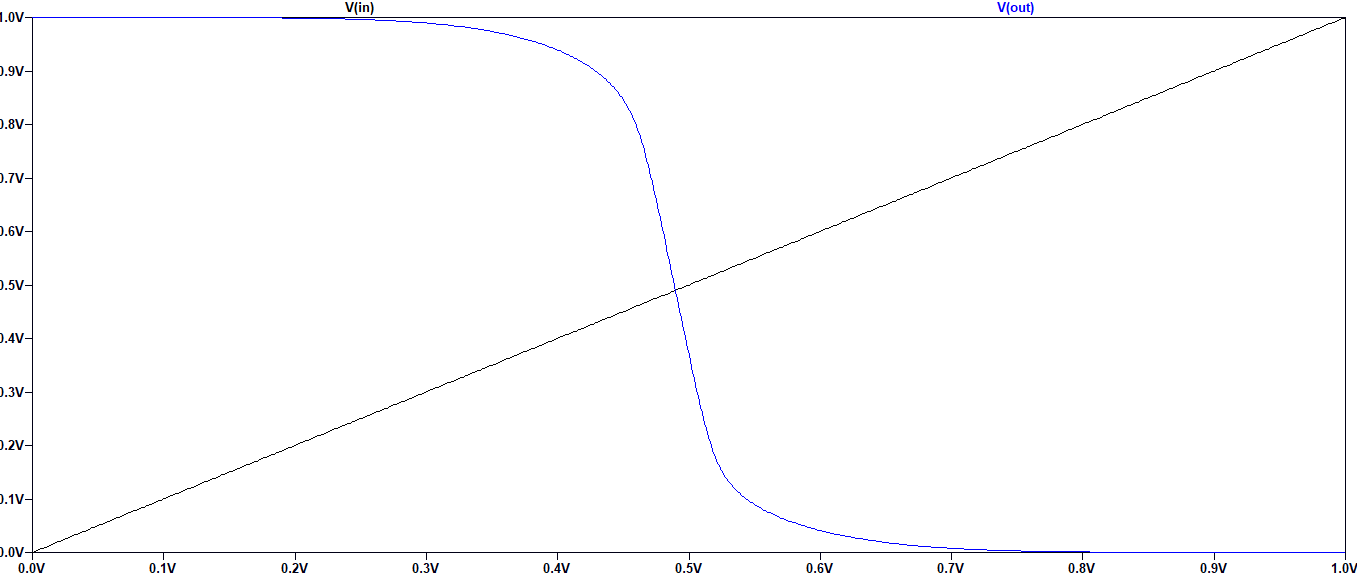
\includegraphics[width=0.8\textwidth]{Imagenes/curvacarac.png}
    \caption{Curva característica del inversor}
    \label{fig:curvacarac}
    \end{figure}
\subsection{Creación del símbolo}

Ahora con el inversor ya creado, procedemos a crear su símbolo, para esto hay que ir al apartado Hierarchy del LTSpice y seleccionar la opción 'Create a New Symbol', luego hay que dibujar el inversor y guardarlo en la carpeta donde esta el esquemático.

   \begin{figure}[H]
    \centering
    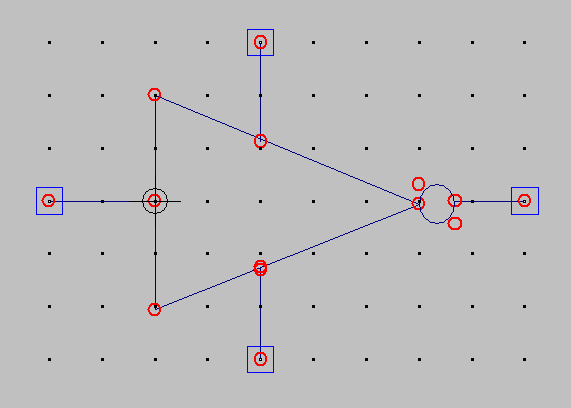
\includegraphics[width=0.8\textwidth]{Imagenes/symbol.png}
    \caption{Creación del símbolo del inversor}
    \label{fig:symbol}
    \end{figure}

\subsection{Simulación transient del inversor}
Ahora en un nuevo archivo armamos un nuevo testbench en el cual colocamos el símbolo del inversor ya como si fuera un inversor individual, el esquematico es el siguiente:

   \begin{figure}[H]
    \centering
    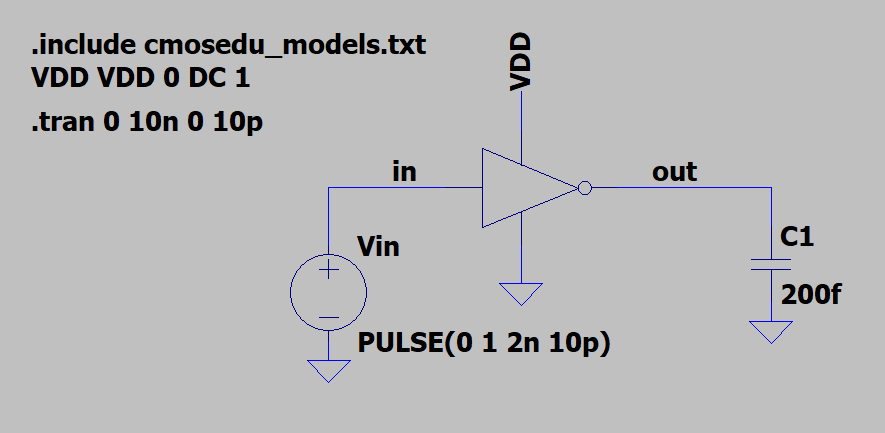
\includegraphics[width=0.8\textwidth]{Imagenes/esquematico 2.png}
    \caption{Esquemático de prueba del inversor}
    \label{fig:esquematico 2}
    \end{figure}

    Se eligió una carga de pequeño valor para verificar el funcionamiento del inversor, la gráfica obtenida fue la siguiente:

   \begin{figure}[H]
    \centering
    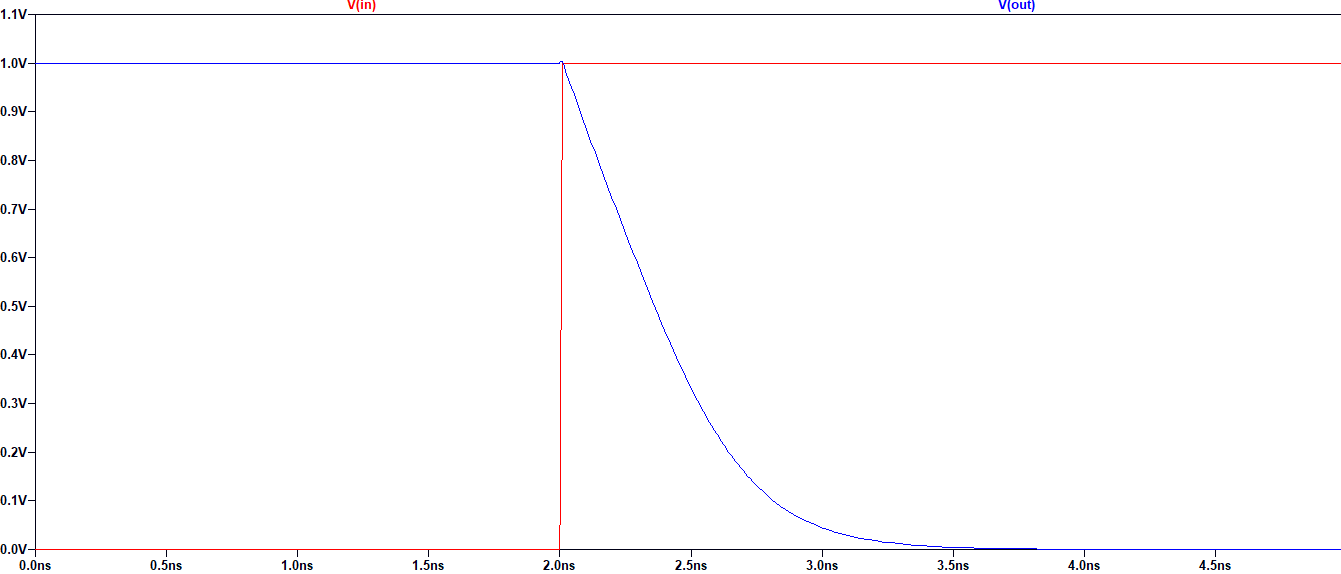
\includegraphics[width=1\textwidth]{Imagenes/resultado1.png}
    \caption{Simulación transient para un solo inversor}
    \label{fig:resultado1}
    \end{figure}

\section{Simulación del Oscilador de Anillo}

\subsection{Simulación sin carga}


Ahora en un nuevo esquemático armamos el Oscilador de Anillo utilizando 13 inversores, pero en este caso no se le colocara capacitores de carga par verificar su funcionamiento, el esquemático es el siguiente:

\begin{figure}[H]
    \centering
    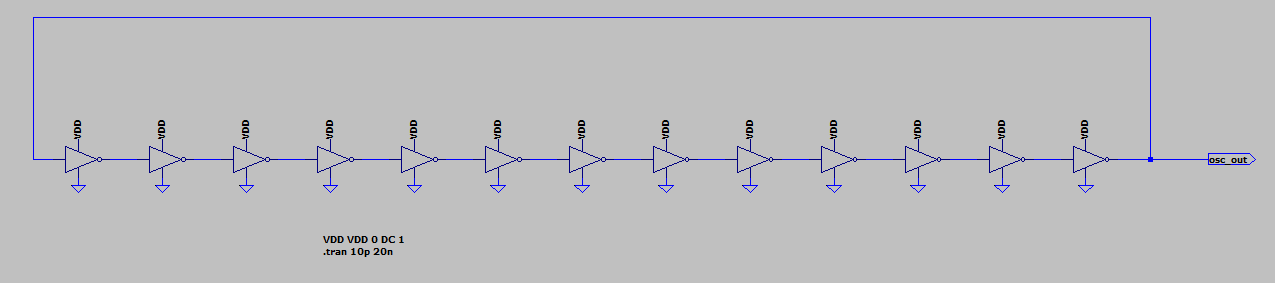
\includegraphics[width=1\textwidth]{Imagenes/esquematico 3.png}
    \caption{Esquemático de un Oscilador de anillo sin carga}
    \label{fig:esquematico 3}
    \end{figure}
Se utilizaron los inversores creados anteriormente, los resultados obtenidos fueron:




\begin{figure}[H]
    \centering
    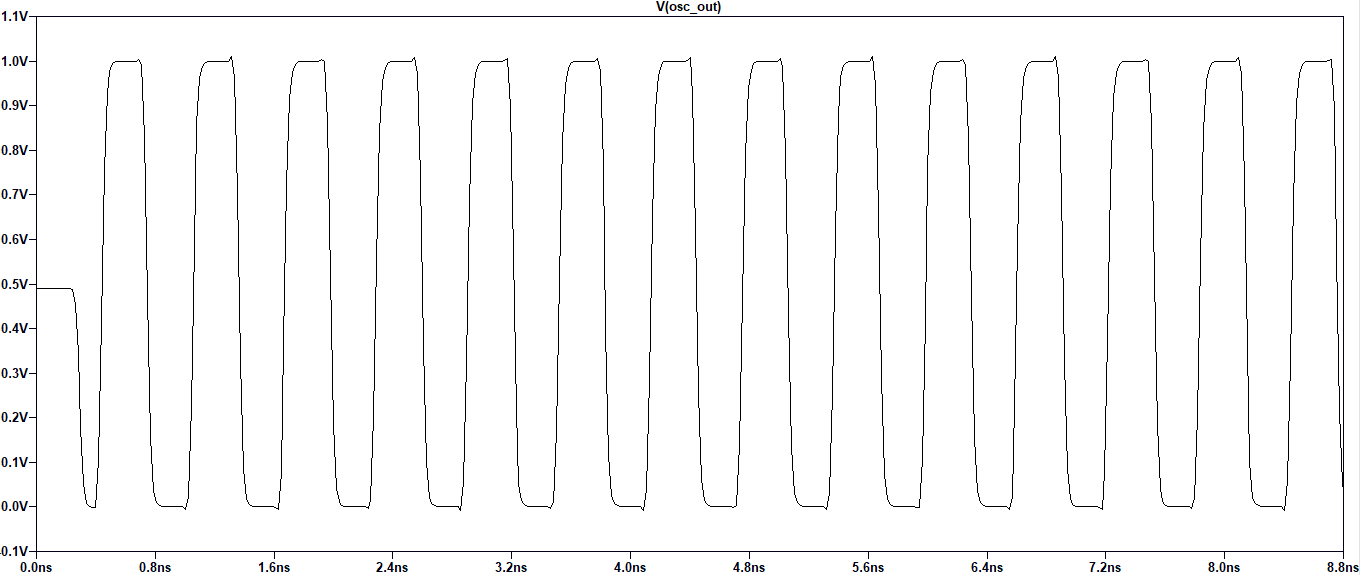
\includegraphics[width=1\textwidth]{Imagenes/resultado2.png}
    \caption{Simulación transient para Oscilador de anillo}
    \label{fig:resultado2}
    \end{figure}



\begin{figure}[H]
    \centering
    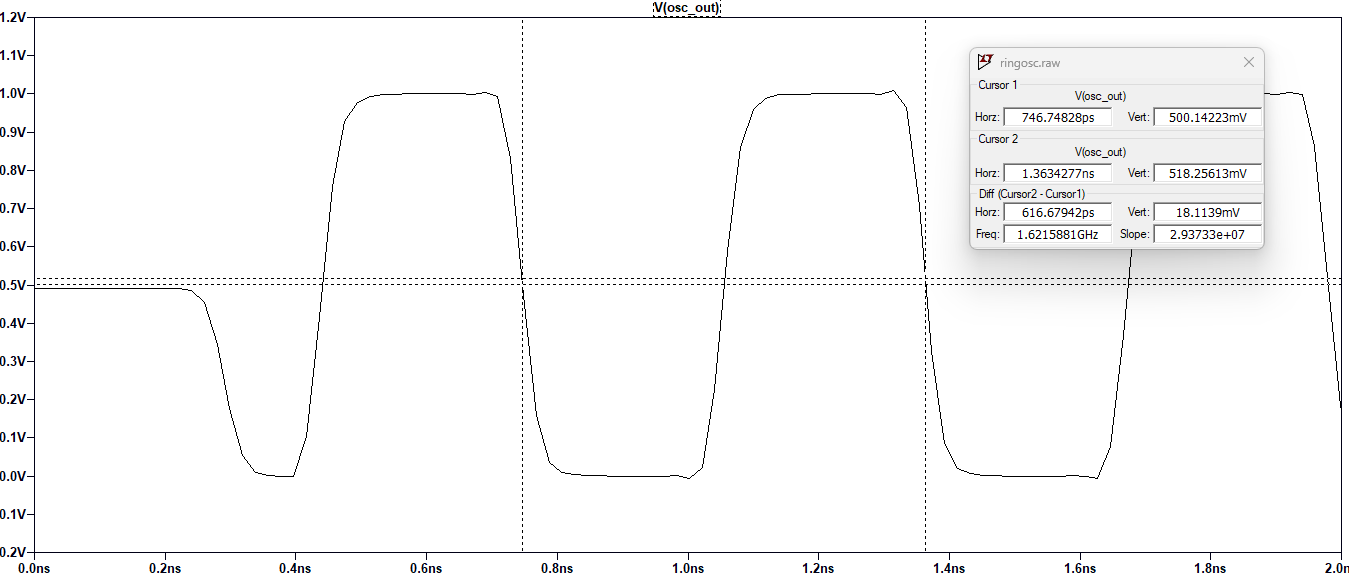
\includegraphics[width=1\textwidth]{Imagenes/resultado3.png}
    \caption{Detalle de la simulación}
    \label{fig:resultado3}
    \end{figure}

Se puede observar que sin colocar los capacitores de carga la frecuencia de oscilación fue de:

\begin{equation}
f_{\text{simulada}} = 1.82 \, \mathrm{GHz}
\end{equation}

\subsection{Simulación con carga}

Ahora se les colocaron las cargas a los inversores, el esquemático es el siguiente
\begin{figure}[H]
    \centering
    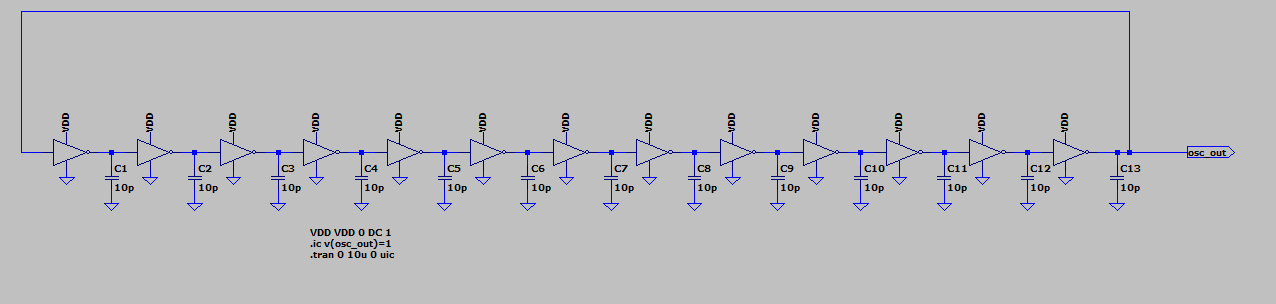
\includegraphics[width=1\textwidth]{Imagenes/esquematico 4.png}
    \caption{Esquemático de un Oscilador de anillo}
    \label{fig:esquematico 4}
    \end{figure}

Los resultados obtenidos fueron los siguientes:

\begin{figure}[H]
    \centering
    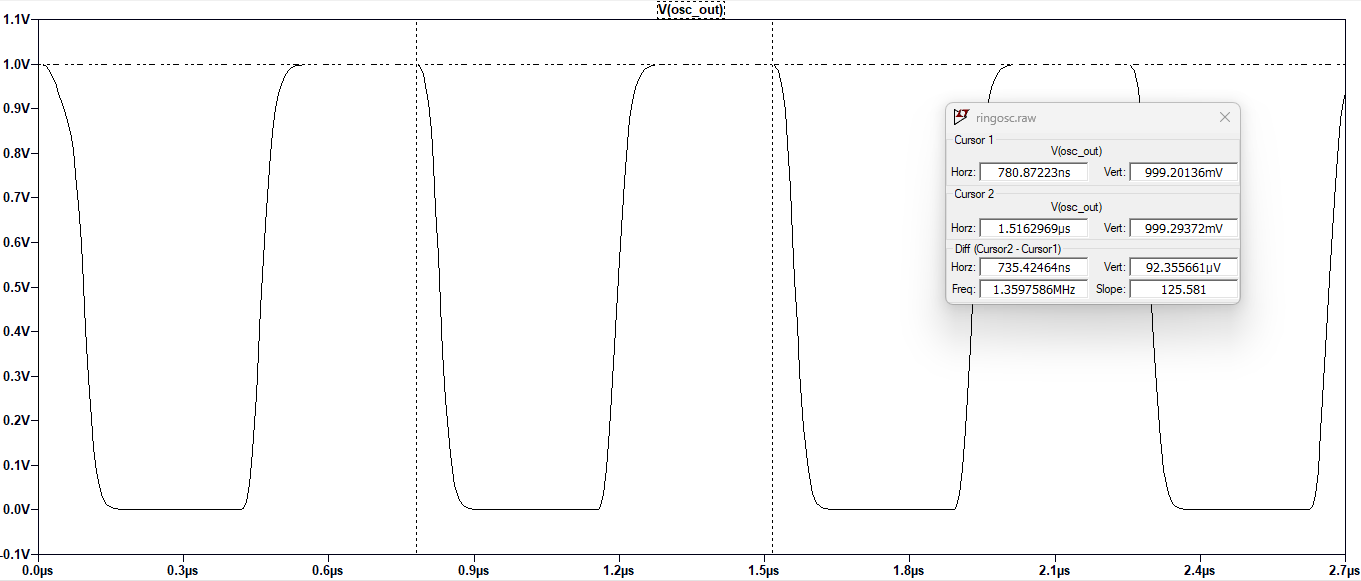
\includegraphics[width=1\textwidth]{Imagenes/resultado4.png}
    \caption{Simulación del oscilador de anillo con carga}
    \label{fig:resultado4}
    \end{figure}

Ahora con los capacitores de carga colocados se puede observar que la frecuencia de oscilación cae significativamente, el valor resultante de frecuencia de oscilación es de:

\begin{equation}
f_{\text{simulada}} = 1.36 \, \mathrm{MHz}
\end{equation}

\section{Interpretación de los resultados}
\subsection{Comparación entre lo medido y lo calculado}

A continuación se presenta un cuadro que compara la frecuencia de oscilación obtenida y la calculada de forma teórica
\begin{table}[H]
\centering
\begin{tabular}{|c|c|c|}
\hline
 & $Teorico$ & $Medido$\\ \hline
\textbf{Frecuencia} & 3.85 Mhz & 1.36 Mhz \\ \hline
\end{tabular}
\caption{Comparación entre valor calculado y medido}
\label{tab:two_by_two}
\end{table}

Al calcular de forma teórica la frecuencia de oscilación con un tiempo de propagación de 10ns, nos queda una frecuencia de oscilación de 3.85Mhz

Esta diferencia es muy significativa, y sucede porque el tiempo de propagación es distinto a 10ns, al tener un tamaño fijo los transistores tienen un tiempo de propagación fijo, para llegar a este valor habría que aumentar su tamaño, reduciendo su tiempo de propagación.

\subsection{Corrección en el calculo de la frecuencia de oscilación}


Lo que se hizo fue medir el tiempo de propagación de un inversor con carga de 10pf y luego se calculo nuevamente la frecuencia teórica.

La simulación transient del inversor con la carga nueva da como resultado:

\begin{figure}[H]
    \centering
    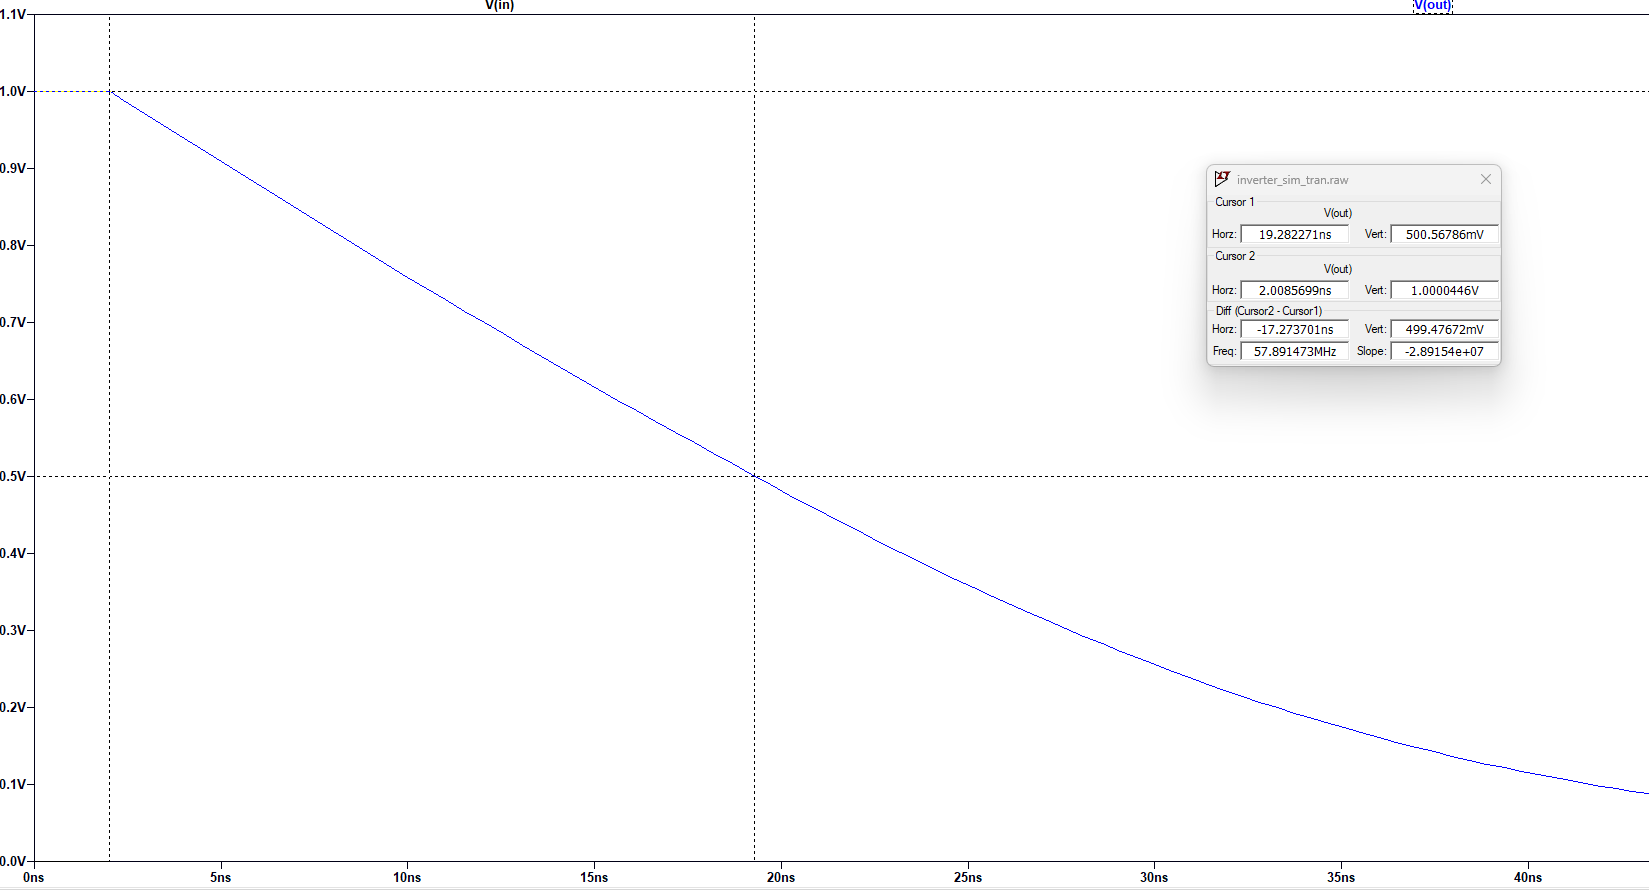
\includegraphics[width=1\textwidth]{Imagenes/Resultado5.png}
    \caption{Simulación del oscilador de anillo con carga de 10 pf}
    \label{fig:resultado5}
    \end{figure}

El valor del tiempo de propagación medido fue de :
    \begin{equation}
t_{\text{prop}} = 17.2 \, \mathrm{ps}
\end{equation}

Calculando nuevamente la frecuencia de oscilación teórica nos queda:

\[
f = \frac{1}{2 \cdot 13 \cdot 17.2 \, \mathrm{ns}} = \frac{1}{260 \, \mathrm{ns}} \approx 2.23 \, \mathrm{MHz}
\]

\begin{table}[H]
\centering
\begin{tabular}{|c|c|c|}
\hline
 & $Teorico$ & $Medido$\\ \hline
\textbf{Frecuencia} & 2.23 Mhz & 1.36 Mhz \\ \hline
\end{tabular}
\caption{Comparación entre valor calculado y medido}
\label{tab:two_by_two2}
\end{table}

Se puede observar que el error se redujo significativamente

\section{Conclusión}

En este trabajo, se estudió el diseño y la simulación de un oscilador de anillo basado en 13 inversores CMOS utilizando LTspice. A través de un análisis teórico, se determinó la frecuencia esperada del circuito, calculada en \( f_{\text{teórica}} = 2.23 \, \mathrm{MHz} \), considerando un tiempo de propagación \( t_p = 17.2 \, \mathrm{ns} \) y las especificaciones del diseño.

Posteriormente, mediante la simulación del circuito en LTspice, se obtuvo una frecuencia de oscilación simulada de \( f_{\text{simulada}} = 1.36 \, \mathrm{MHz} \), mostrando un excelente acuerdo con los cálculos teóricos. Las pequeñas discrepancias entre los valores teóricos y simulados se atribuyen a efectos parasitarios, como las capacidades no ideales y los retardos adicionales que no fueron considerados en el modelo analítico.

Mediante este trabajo pudimos comprender aspectos de la microelectrónica, ya sea desde el dimensionamiento de los transistores hasta la importancia de la carga de los mismos. al aumentar la carga la frecuencia de oscilación cae fuertemente

También aprendimos a crear símbolos en LTSpice, y a configurar los parámetros del circuito modificando las dimensiones de los transistores

Este ejercicio nos permitió comprender el funcionamiento de los osciladores de anillo, desde la caracterización inicial de un inversor CMOS hasta el análisis completo del circuito oscilador. 

Finalmente, el oscilador de anillo nos aprecio un diseño simple y eficiente, con aplicaciones prácticas en sistemas digitales, como generadores de reloj y medición de tiempos de propagación en tecnología CMOS. 


\end{document}
% ------------------------------------- Desarrollo ---------------------------------